\chapter{Diseño de la solución}\label{cap:diseño}

\section{Introducción}
La base de datos se ha estructurado como un grafo multimodelo denominado \texttt{RedLogistica}. A diferencia de las bases de datos relacionales estándar, este modelo me permite recorrer conexiones logísticas con una eficiencia de orden de complejidad mucho menor.

\section{Modelo de Datos y Diagrama}
La organización lógica de las colecciones diseñadas en ArangoDB es la siguiente:
\begin{itemize}
    \item \textbf{Vértices (Documentos):} \texttt{Almacenes} y \texttt{Productos}.
    \item \textbf{Aristas (Edges):} \texttt{Rutas} (conecta almacenes entre sí, incluyendo el atributo \texttt{distancia\_km}) y \texttt{Stock\_en} (conecta productos con almacenes, incluyendo el atributo de \texttt{cantidad}).
\end{itemize}

En la Figura \ref{fig:grafo_db} se ilustra la topología de la base de datos mediante un diagrama conceptual.

\begin{figure}[htp]
    \centering
    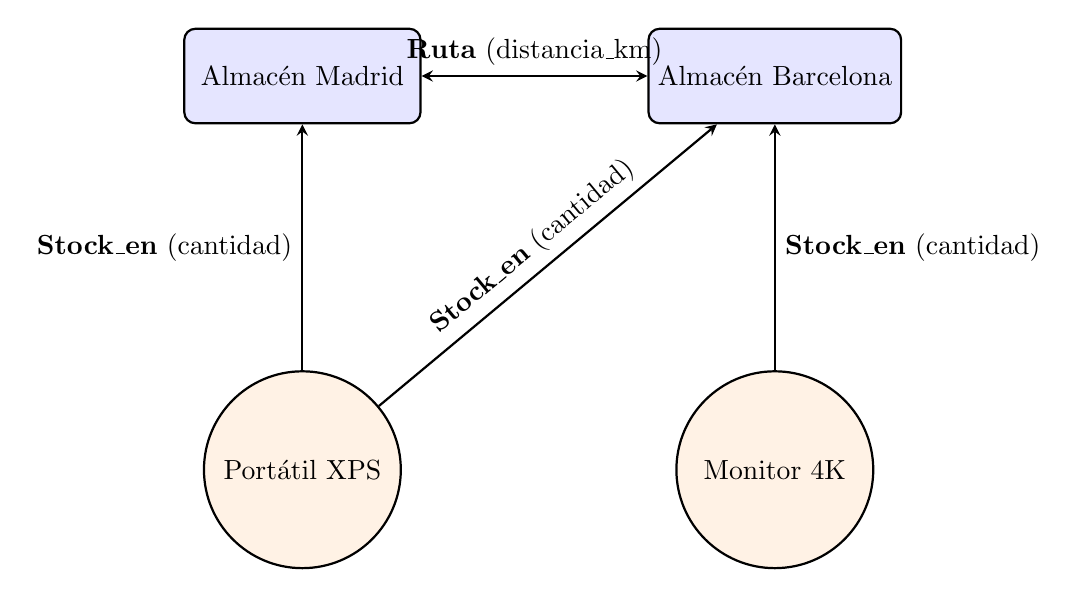
\begin{tikzpicture}[node distance=4cm, auto, thick, >=stealth]
        % Definición de estilos
        \tikzstyle{nodoAlmacen} = [draw, rectangle, rounded corners, fill=blue!10, minimum width=3cm, minimum height=1.2cm, text centered]
        \tikzstyle{nodoProducto} = [draw, circle, fill=orange!10, minimum size=2.5cm, text centered]

        % Nodos Almacenes
        \node[nodoAlmacen] (almacenMadrid) {Almacén Madrid};
        \node[nodoAlmacen, right of=almacenMadrid, xshift=2cm] (almacenBarna) {Almacén Barcelona};
        
        % Nodos Productos
        \node[nodoProducto, below of=almacenMadrid, yshift=-1cm] (prodPortatil) {Portátil XPS};
        \node[nodoProducto, below of=almacenBarna, yshift=-1cm] (prodMonitor) {Monitor 4K};

        % Aristas
        \draw[<->] (almacenMadrid) -- node[above] {\textbf{Ruta} (distancia\_km)} (almacenBarna);
        \draw[->] (prodPortatil) -- node[left] {\textbf{Stock\_en} (cantidad)} (almacenMadrid);
        \draw[->] (prodMonitor) -- node[right] {\textbf{Stock\_en} (cantidad)} (almacenBarna);
        \draw[->] (prodPortatil) -- node[above, sloped] {\textbf{Stock\_en} (cantidad)} (almacenBarna);
    \end{tikzpicture}
    \caption{Diagrama topológico del grafo \texttt{RedLogistica} y sus relaciones.}
    \label{fig:grafo_db}
\end{figure}

\section{Decisiones de Diseño: Integridad en Grafos}
Una decisión arquitectónica crítica a la que tuve que enfrentarme fue la gestión de la integridad referencial. Dado que ArangoDB no impone restricciones rígidas de borrado en cascada de la misma forma que un motor SQL, tuve que implementar lógica AQL manual transaccional. Esto garantiza que, si se elimina un almacén del sistema por necesidades de negocio, se supriman simultáneamente todas sus rutas adyacentes y registros de stock vinculados, previniendo la existencia de "aristas huérfanas" que pudieran corromper consultas futuras.

\section{Conclusiones}
El diseño propuesto explota las ventajas de los grafos nativos para resolver un problema de red complejo, garantizando al mismo tiempo la consistencia de los datos mediante una capa lógica de control implementada directamente en el código de backend.